%\documentclass[a4paper,12pt,oneside,draft]{article}
\documentclass[a4paper,12pt,oneside]{article}

% In the original writelatex tamplate
\usepackage[english]{babel}
\usepackage[utf8]{inputenc}
\usepackage{amsmath}
\usepackage{graphics}
\usepackage[colorinlistoftodos]{todonotes}

% By LoCigno
\usepackage{times}
\usepackage{graphicx}
\usepackage{subfigure}
\usepackage{csvsimple}
\usepackage{color}
\usepackage{url}
\usepackage{hyperref} 
\usepackage{cleveref}

% By Davide
\usepackage{comment}
\usepackage{booktabs}
\usepackage{color}

%Variables macros
\newcommand{\DefineVar}[2]{%
  \expandafter\newcommand\csname var-#1\endcsname{#2}%
} 
\newcommand{\var}[1]{\csname var-#1\endcsname}

\usepackage{courier}
\newcommand{\mono}[1]{\texttt{#1}}

\title{Controller design for Lego Mindstorm motor}

\author{Diego Verona, Aliaksandr Siarohin, Mattia Digilio}

\date{\today}

% By Diego
\newtheorem{thm}[equation]{Theorem}
\usepackage[outdir=./]{epstopdf}
\usepackage{float}

\begin{document}
%\maketitle
\makeatletter  % populates \@title, \@author, \@date
\begin{titlepage}
      \centering
      ~~~~~~~~~~~~~\\[-30mm]
      \includegraphics[keepaspectratio=true, width=7cm]{bg_eng_1r.jpg} \\[10mm]

     {
     \large \bfseries Master Degree in Computer Science\\[3mm] 
     Applied Robotics\\[3mm]
     AA 2015-2016
     }\\[10mm]

     %--------------------------------
     % Set the title, author, and date
     % 

     \vspace{0.5cm}
     {
     \Large \bfseries \textcolor{blue}{\@title} \par
     }
     \vspace{0.5cm}
%      {
%      \large {Group N. 1} \par
%      }
     \vspace{0.2cm}

     {\large {\@author}}
     \\ \vspace{.2cm}
     \@date

     \vspace{0.6cm}

    %-----------------------------------

\begin{abstract}

\textit{
  Report for the second assignment on Applied robotics: design and implement controller for the Lego NXT motor.\\In this report we show our controller, describe it properties and describe it digital implementation.
}


\end{abstract}

\end{titlepage}

\section{General definition}

\begin{thm}
\textbf{Root locus}. The \texttt{root locus}, or \texttt{Evans locus}, is a graphical method that
depicts the curves of the roots of the denominator of the closed loop transfer function in the complex plane
(sometimes called Argand plane or Gauss plane). The curves are parameterized by a parameter, typically the
gain of the loop  \footnote{\url{http://disi.unitn.it/~palopoli/courses/ECL/RootLocus.pdf}}
\end{thm}
\begin{thm}
\textbf{Closed-loop transfer function}. A closed-loop transfer function in control theory is a mathematical expression (algorithm) describing the net result of the effects of a closed (feedback) loop on the input signal to the circuits enclosed by the loop. \footnote{\url{https://en.wikipedia.org/wiki/Closed-loop_transfer_function}}
\end{thm}

\begin{figure}[h]
	\vspace{-1.5em}
	\centering
	\includegraphics[width=\columnwidth]{./closed_loop_controller.png}
	\vspace{-1.5em}
	\caption{Closed loop with controller}
	\label{fig:closed_loop_controller}
	\vspace{-2em}
\end{figure}

\section{Design of continues time controller}
\subsection{Controller requirments}
The contoller should has:
\begin{itemize}
\item stady state tracking error = 0
\item overshot $<$ 20\%
\item settling time $<$ 0.4s
\end{itemize}
Overshot requirement on root locus plot is shown by the following formula:
\begin{equation}
\frac{Re}{Im} = \frac{\xi}{\sqrt{1-\xi^{2}}} = \pm\frac{ln{0.2}}{\pi}
\end{equation}

To show settling time requirement, it is possible to use the dominant pool approximation:
\begin{equation}
Re = \frac{ln(\alpha)}{0.4}
\end{equation}

\subsection{Our design}
\begin{equation}
C(s) = \frac{(s+10)^2}{s(s+21)}
\end{equation}
\begin{equation}
K_c = 10
\end{equation}
Root locus can be seen in \cref{fig:root_locus}, and the ideal response to 1(t) in \cref{fig:response}.\\ Results of Scicoslab simulation is shown in different figures:
\begin{itemize}
\item $\Omega$ in \cref{fig:simulation_omega}
\item Power in \cref{fig:simulation_power}
\item Tracking error in \cref{fig:simulation_tracking_err}
\end{itemize}
Code is available in a shared folder\footnote{\url{https://github.com/AliaksandrSiarohin/AppliedRobotics/tree/master/controler}}.

\section{Practical case: vehicle}
Using 2 different motors applied on the NXT brick, it is possible to do a simple modelling of a vehicle. The scope of this simple experiment is to let our model to go straight without any external sensors, but only using the the following implementation of a digital controller.
\begin{figure}[H]
	\vspace{-1em}
	\centering
	\includegraphics[width=\columnwidth]{./vehicle.png}
	\vspace{-1.5em}	
	\caption{Closed loop with controller}
	\label{fig:closed_loop_controller}
	\vspace{-1em}	
\end{figure}
Digital version of controller is obtained using trapezoid rule:
\begin{multline}
y_{k+2} = \frac{1}{4 + 42 * T} (K_cu_{k+2}(4 + 100T^2 + 40T) + K_cu_{k+1}(-8 + 200T^2) \\+ K_cu_{k}(4 - 40T + 100T^2) + 8y_{k+1} - y_{k}(4 - 42*T))
\end{multline}
Speed estimated using exponential average:
\begin{equation}
S(t) = 0.075 * S(t) + (1 - 0.075) * \frac{(Angle(t) - Angle(t-1))}{T}
\end{equation}
Code is available in a shared folder\footnote{\url{https://github.com/AliaksandrSiarohin/AppliedRobotics/tree/master/motor_controller}}.

\begin{figure}
	\centering
	\includegraphics[width=\columnwidth]{../controler/root_locus}
	\caption{Root locus, red lines show constains on overshot and settling time}
	\label{fig:root_locus}
	\centering
	\includegraphics[width=\columnwidth]{../controler/response}
	\caption{response to 1(t).}
	\label{fig:response}
\end{figure}

\begin{figure}
	\centering
	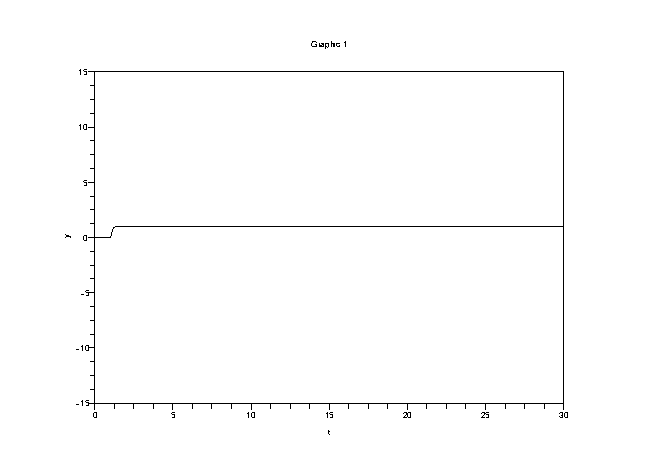
\includegraphics[width=\columnwidth]{../controler/omega.eps}
	\caption{Scicoslab simulation: omega}
	\label{fig:simulation_omega}
	\centering
	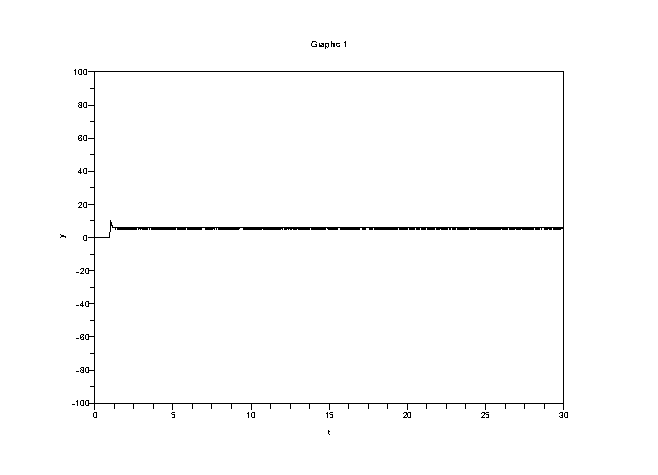
\includegraphics[width=\columnwidth]{../controler/power.eps}
	\caption{Scicoslab simulation: power}
	\label{fig:simulation_power}
\end{figure}
\begin{figure}
	\centering
	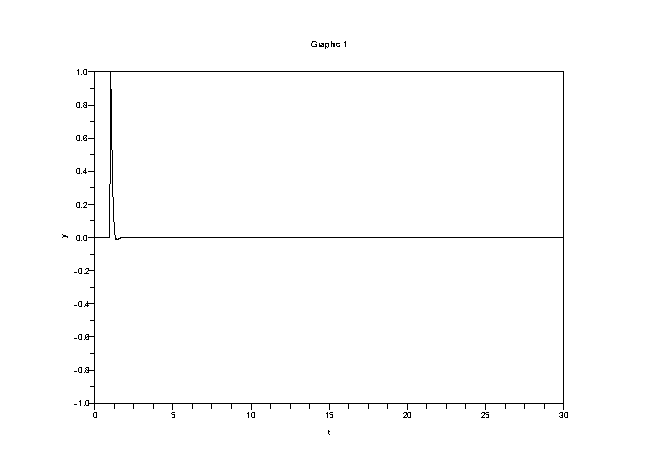
\includegraphics[width=\columnwidth]{../controler/tracking_err.eps}
	\caption{Scicoslab simulation: tracking error}
	\label{fig:simulation_tracking_err}
\end{figure}

\section{Conclusion}


\end{document}